\chapter{Architektura}
\label{cha:architektura}

\section{Platforma}
\label{sec:platforma}
Platformą, którą wybrałem do mojej pracy, jest heterogeniczny układ Intel Cyclone V SoC.
Zawiera on FPGA oraz HPS (Hard Processor System) oparty na procesorze ARM, co umożliwia
podział zadań między hardware i software. Ze względu na przystępną cenę i elastyczność konfiguracji,
układ ten znajduje szerokie zastosowanie w projektach wymagających kompromisu między wydajnością a kosztami,
szczególnie w środowiskach akademickich. W pracy przedstawię, jak efektywnie wykorzystać ten układ do implementacji zaawansowanych algorytmów przetwarzania sygnałów.

\begin{figure}[!htb]
    \centerline{\includegraphics[scale=0.2]{de0-nano-soc.png}}
    \caption{Układ DE0-Nano-SoC (Cyclone V)}
    \label{fig:de0-nano-soc}
\end{figure}

\newpage
\section{Architektura Hardware'u}
\label{sec:architektura-hw}

\begin{figure}[!htb]
    \centerline{\includegraphics[scale=0.5]{hardwareSystemDiagram.png}}
    \caption{Diagram przedstawiający architekturę systemu}
    \label{fig:architektura}
\end{figure}

\newpage
\section{Architektura Software'u}
\label{sec:architektura-sw}

\begin{figure}[!htb]
    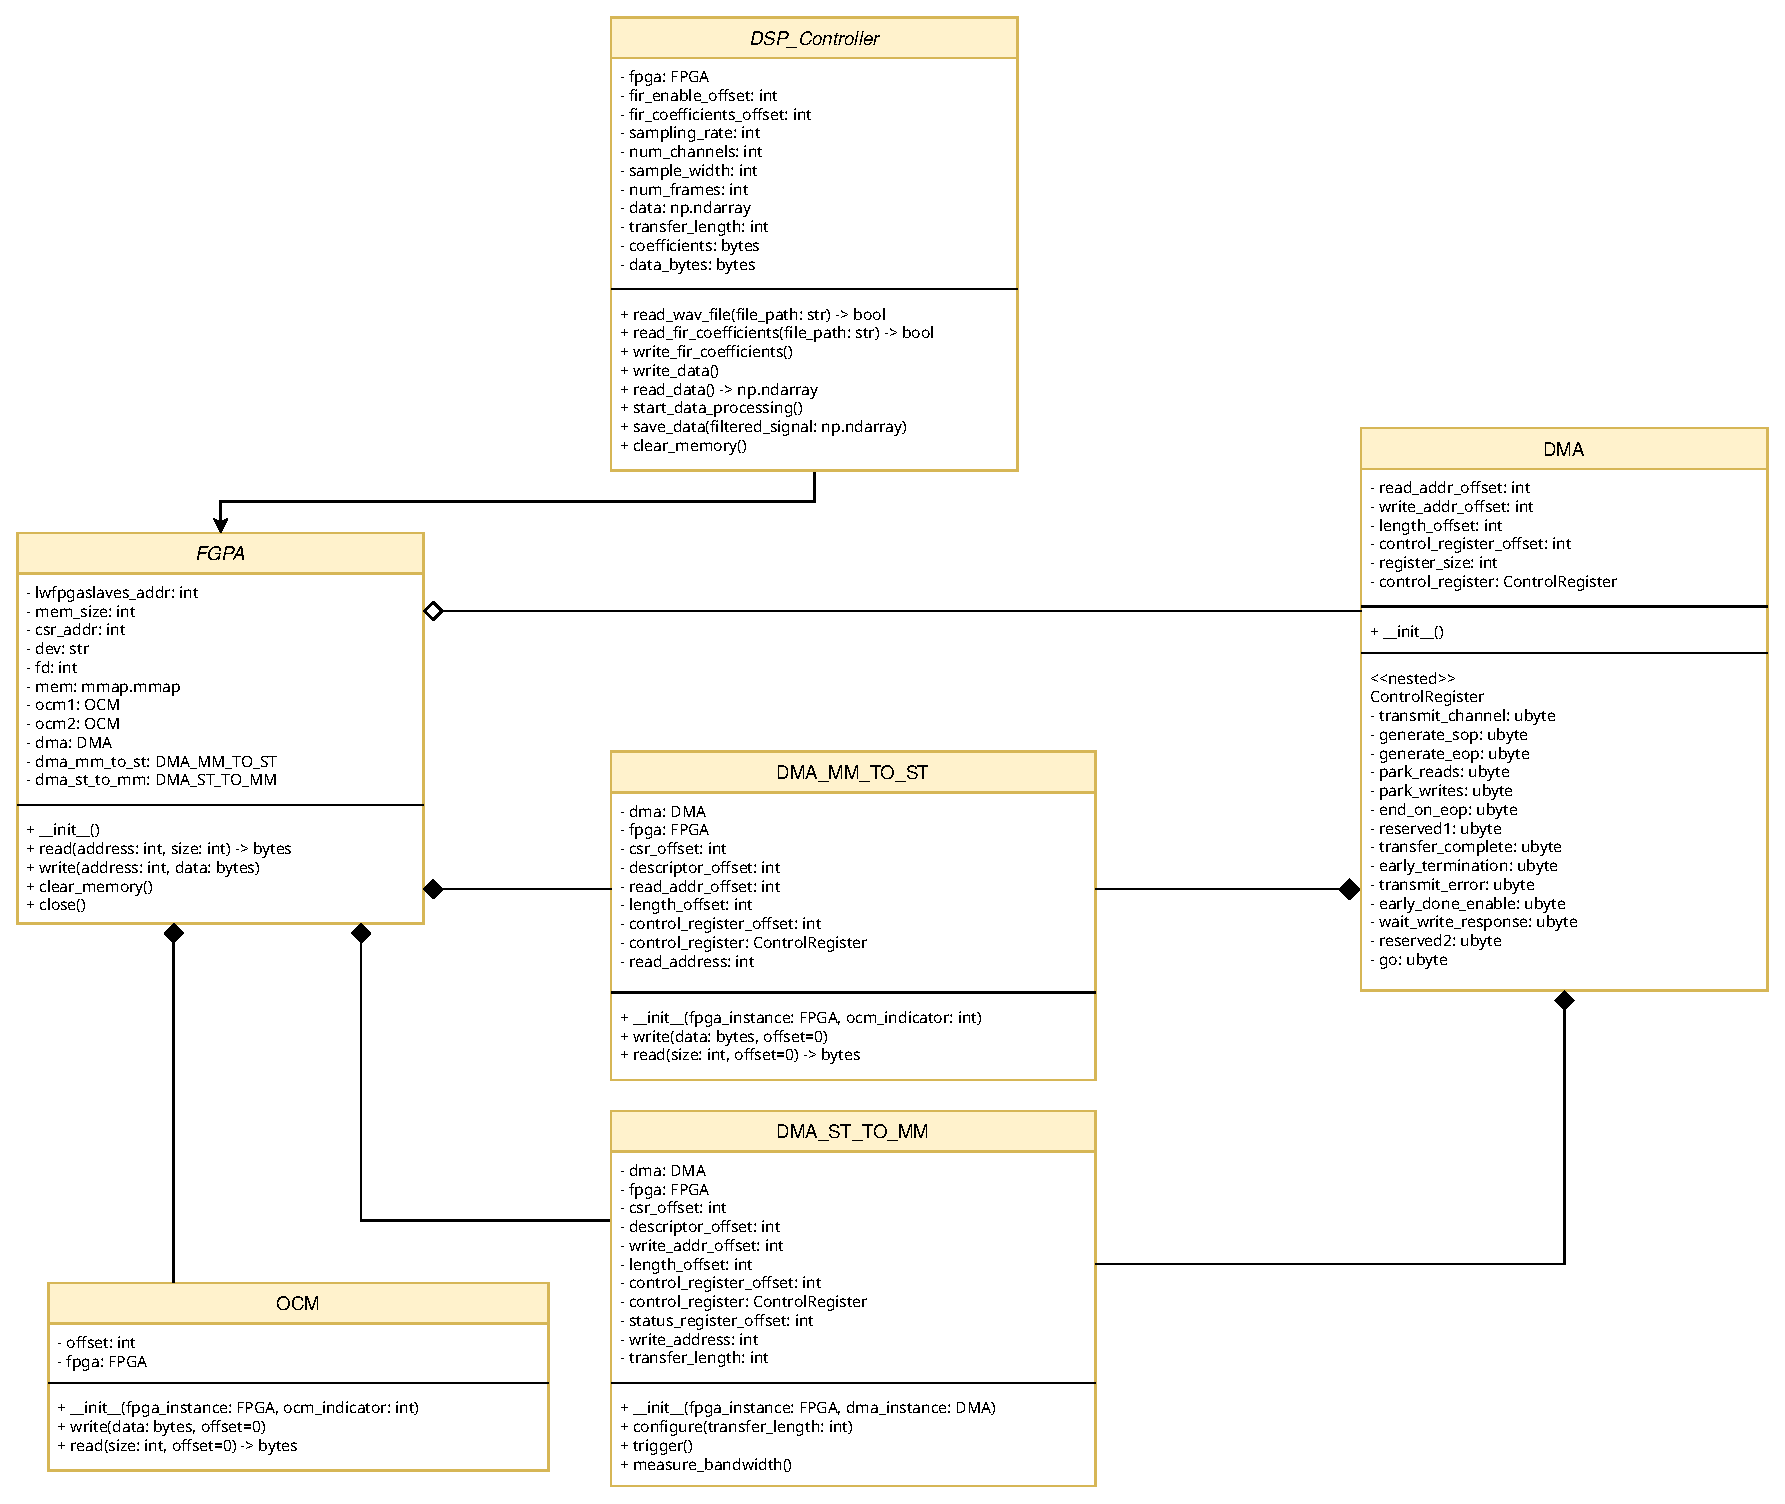
\includegraphics[scale=0.53]{classDiagram.eps}
    \caption{Diagram klas}
    \label{fig:diagram-klas}
\end{figure}



